\documentclass[12pt]{exam}

\newcommand{\ds}{\ensuremath{\displaystyle}}

\usepackage{amsmath,amsfonts, amsthm}
\usepackage{multicol}
\usepackage{multirow}
\usepackage{harpoon}
\renewcommand{\arraystretch}{1.5}

\newcommand{\harpvec}[1]{\overrightharp{\ensuremath{\mathbf{#1}}}}
\newcommand{\vect}[1]{\ensuremath{\mathbf{#1}}}
\newcommand{\<}{\langle}
\renewcommand{\>}{\rangle}
\newcommand{\p}{\partial}

% ref: http://pgfplots.sourceforge.net/gallery.html
% ref: http://tex.stackexchange.com/a/74575/79754
\usepackage{pgfplots}% This uses tikz
\pgfplotsset{compat=newest}% use newest version
\tikzset{LineStyle/.style={smooth, ultra thick, samples=400}}

% \printanswers

\begin{document}

\begin{center}
\fbox{\fbox{\parbox{5.5in}{\centering
MATH 2242 - Fall 2015 - Dr. Clontz - Test 1
}}}
\end{center}
\vspace{0.1in}
\makebox[\textwidth]{
  Name:\enspace\hrulefill\hrulefill\hrulefill\space
  Section:\enspace\hrulefill\space
}

\vspace{12pt}

\begin{itemize}
  \item This test is worth 250 points toward your overall grade.
        Each problem is labeled with its value toward this total.
  \item On multiple choice problems, you do not need to show your work. No
        partial credit will be given.
  \item On full response problems, show all of your work and give a
        complete solution. When in doubt, don't skip any steps. Partial
        credit will be given at the discretion of the instructor.
  \item This exam is open notes, provided that these notes are completely
        in your own handwriting. The professor may take up notes you use
        with your test and return them after the test is graded.
  \item Tests submitted after the end of 70 minutes will be deducted 25 points,
        with 25 more points deducted every following minute.
\end{itemize}

\newpage

\begin{center}
  \textbf{Multiple Choice (100 points total)}
\end{center}

\begin{questions}

\setcounter{question}{0}
\question[20]
Evaluate \(AB\) given
\[
  AB
    =
  \left[
  \begin{matrix}
     1 &  2 &  0\\
    -3 &  0 &  4
  \end{matrix}
  \right]
  \left[
  \begin{matrix}
     3 & -1 \\
     0 &  1 \\
    -1 &  4
  \end{matrix}
  \right]
\]


\begin{checkboxes}
\choice \(
  \left[
  \begin{matrix}
     0  & -11 \\
     4 & 2
  \end{matrix}
  \right]
\)
\choice \(
  \left[
  \begin{matrix}
     3  &  1 \\
    -13 & 19
  \end{matrix}
  \right]
\)
\choice \(
  \left[
  \begin{matrix}
     3  &  0 & 0 \\
     3 &  0 & 8 \\
  \end{matrix}
  \right]
\)
\choice \(
  \left[
  \begin{matrix}
     -1  &  2 & 0 \\
     -9 &  0 & -4 \\
  \end{matrix}
  \right]
\)
\choice None of these
\end{checkboxes}

\vfill

\question[20]
Compute \(\frac{\p f}{\p y}\) where \(f:\mathbb R^3\to\mathbb R\) is
defined by \(f(x,y,z) = e^{xy}-2yz^3 \).

\begin{checkboxes}
\choice \(\frac{\p f}{\p y}=xe^{xy}-2z^3\)
\choice \(\frac{\p f}{\p y}=xye^{xy}-6yz^2\)
\choice \(\frac{\p f}{\p y}=\log(xy)-2yz^2\)
\choice \(\frac{\p f}{\p y}=e^x + ye^y -6z^2\)
\choice None of these
\end{checkboxes}

\vfill
\newpage

\question[20]
Let \(\vect f(x,y)=\<x^2,y-x\>\) and \(\vect g(r,s,t)=\<rs,e^t\>\).
Which of these is equal to \(\vect D[\vect f\circ\vect g]\)?

\begin{checkboxes}
\choice \(
  \left[
  \begin{matrix}
     1 & 2rs\\
     -1 & 0
  \end{matrix}
  \right]
  \left[
  \begin{matrix}
     s & 0 & e^t\\
     r & 0 & 0
  \end{matrix}
  \right]
\)
\choice \(
  \left[
  \begin{matrix}
     0 & 2rs\\
     -1 & 1
  \end{matrix}
  \right]
  \left[
  \begin{matrix}
     0 & 0 & e^t\\
     s & r & 0
  \end{matrix}
  \right]
\)
\choice \(
  \left[
  \begin{matrix}
     2rs & 0\\
     -1 & 1
  \end{matrix}
  \right]
  \left[
  \begin{matrix}
     s & r & 0\\
     0 & 0 & e^t
  \end{matrix}
  \right]
\)
\choice \(
  \left[
  \begin{matrix}
     -1 & 1\\
     2rs & 0
  \end{matrix}
  \right]
  \left[
  \begin{matrix}
     r & s & 0\\
     e^t & 0 & 0
  \end{matrix}
  \right]
\)
\choice None of these.
\end{checkboxes}

\vfill

\question[20]
Which of these functions is the linear approximation \(L(x,y,z)\) of
\(f(x,y,z)\) near \((1,0,-2)\) given by Taylor's Theorem?
\begin{checkboxes}
  \choice \(L(x,y,z) = f(1,0,-2)+\frac{\p f}{\p x}(1,0,-2)(x-1)+\frac{\p f}{\p y}(1,0,-2)(y)+\frac{\p f}{\p z}(1,0,-2)(z+2)\)
  \choice \(L(x,y,z) = \sum_{i=1}^4\frac{\p f}{\p x_i}(1,0,-2)(x_i-1)\)
  \choice \(L(x,y,z) = \vect D[f](1,0,-2)\vect D[L]\)
  \choice \(L(x,y) = f(1,0,-2)\frac{\p f}{\p x}(1,0,-2)\frac{\p f}{\p y}(1,0,-2)\frac{\p f}{\p z}(1,0,-2)(x+y+z-1)\)
  \choice None of these
\end{checkboxes}

\vfill
\newpage

\question[20]
Which of the following vector field plots was generated from the gradient
of \(f(x,y)=x^2+3xy^2\)? (Note that the plots are scaled down by a factor of
20, and zero vectors are shown as arrowheads.)

\begin{multicols}{2}
\begin{checkboxes}
  \choice
    \fbox{
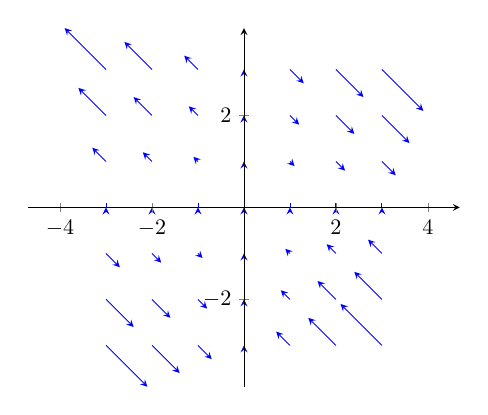
\begin{tikzpicture}[scale=0.8]
\begin{axis}[
        axis equal,
        axis lines=middle,
        domain=-3:3,
        view={0}{90},
]
\addplot3[blue,quiver={
u={2*x*y},
v={-2*x*y},
scale arrows=0.05,
},
-stealth,
samples=7]
{0};
\end{axis}
\end{tikzpicture}
    }
  \choice
    \fbox{
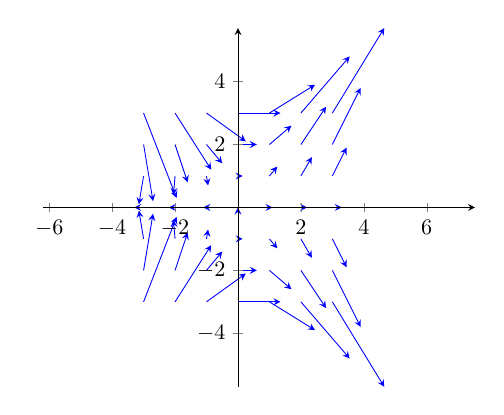
\begin{tikzpicture}[scale=0.8]
\begin{axis}[
        axis equal,
        axis lines=middle,
        domain=-3:3,
        view={0}{90},
]
\addplot3[blue,quiver={
u={2*x+3*y^2},
v={6*x*y},
scale arrows=0.05,
},
-stealth,
samples=7]
{0};
\end{axis}
\end{tikzpicture}
    }
  \choice
    \fbox{
\begin{tikzpicture}[scale=0.8]
\begin{axis}[
        axis equal,
        axis lines=middle,
        domain=-3:3,
        view={0}{90},
]
\addplot3[blue,quiver={
u={x+y},
v={x*y-3},
scale arrows=0.05,
},
-stealth,
samples=7]
{0};
\end{axis}
\end{tikzpicture}
    }
  \choice
    \fbox{
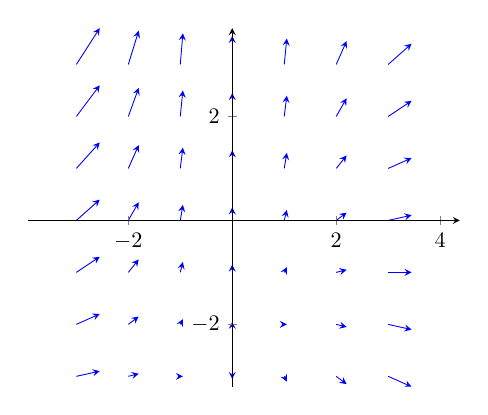
\begin{tikzpicture}[scale=0.8]
\begin{axis}[
        axis equal,
        axis lines=middle,
        domain=-3:3,
        view={0}{90},
]
\addplot3[blue,quiver={
u={x^2},
v={2*y-x+5},
scale arrows=0.05,
},
-stealth,
samples=7]
{0};
\end{axis}
\end{tikzpicture}
    }
\end{checkboxes}
\end{multicols}

\end{questions}





\vfill
\newpage






\begin{center}
  \textbf{Full Response (150 points total)}
\end{center}

\begin{questions}

\setcounter{question}{5}

\question[30]
  Verify the triangle inequality \(\|\vect x+\vect y\|\leq\|\vect x\|+\|\vect y\|\)
  where \(\vect x=\<1,2,2,-4\>\) and \(\vect y =\<0,3,0,4\>\).

  \vfill



\newpage

\question[30]
  Use the fact that \(\vect f:\mathbb R^2\to\mathbb R^2\)
  defined by \(\vect f(x,y)=\<x+y^2,2xy\>\) is a differentiable
  function to explain why
  \[
    \vect f(2.1,-1.1)
      \approx
    \<3,-4\>
      +
    \left[
    \begin{matrix}
      1 & -2 \\
      -2 & 4
    \end{matrix}
    \right]
    \<0.1,-0.1\>
      =
    \<3.3,-4.6\>
  \]

  \vfill



\newpage

\question[30]
  Suppose the temperature at position \((x,y,z)\) is given by
  \(T(x,y,z)=4x^2+4y^2+z^2\). If a particle moves around the curve
  \(\vect c(t)=\<\sin t,-\cos t,2t\>\), describe
  \begin{itemize}
    \item the temperature
  of the particle, \((T\circ\vect c)(t)\)
  \vfill
    \item the rate at which temperature is changing with respect to \(t\),
  \(\frac{d}{dt}[T\circ\vect c](t)\)
  \vfill
  \end{itemize}


\newpage

\question[30]
  What condition(s) must a flow line fitting the vector field
  \(\vect F=\<1,2x\>\) satisfy? Find one such flow line.


\newpage

\question[30]
  Prove \(\textrm{div}(f\vect F)=f\textrm{div}(\vect F)+\vect F\cdot\nabla f\)
  for \(f:\mathbb R^n\to\mathbb R\) and \(\vect F:\mathbb R^n\to\mathbb R^n\).

  (Recall that \(\textrm{div}(\vect G)=\sum_{i=1}^{n}\frac{\p G_i}{\p x_i}\)
  and \(\nabla g=\<\frac{\p g_1}{\p x_1},\dots,\frac{\p g_n}{\p x_n}\>\).)

  Or, for half credit, verify that theorem for \(f(x,y)=x^2+3y\) and
  \(\vect F=\<2x^2y,x+y\>\).

\end{questions}

\end{document}